\chapter{Entorno de desarrollo \textit{NES}}\label{ch:entorno-de-desarrollo-nes}

En este capítulo se abordará el análisis del desarrollo de \textit{NES4JAMS},
un componente que aporta a \textit{JAMS} un entorno de desarrollo
integrado para la creación de videojuegos para la consola
\textit{NES}.
Gracias a la arquitectura de \textit{JAMS}, este componente
aprovechará muchas de las características creadas
para el entorno de desarrollo \textit{MIPS32} presente
por defecto en la aplicación.
Este entorno de desarrollo consistirá en un editor
de texto, un ensamblador y un simulador.


\section{Creación de un proyecto}\label{sec:creacion-de-un-proyecto}

\begin{figure}[h]
    \centering
    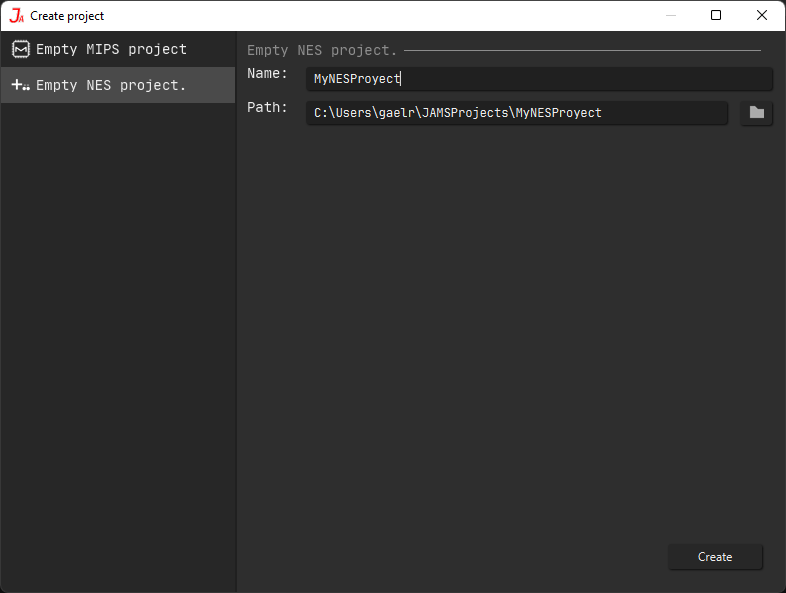
\includegraphics[width=0.85\textwidth]{images/nes/nes-project-creation}
    %% Óscar: he cambiado el width de 0.8 a 0.85 para que no se quede
    %% una línea sola al final, que queda fatal.
    \caption{Creación de un proyecto \textit{NES}}
    \label{fig:nes-project-creation}
\end{figure}

\textit{NES4JAMS} añade a \emph{JAMS} un nuevo tipo de proyecto
que incorpora todas las herramientas para el desarrollo
de videojuegos para \textit{NES}.
Los usuarios podrán crear nuevos proyectos de este tipo
desde el menú de creación de proyectos.
Como los proyectos de \textit{NES} están destinados
a una consola muy específica, el usuario solo debe
especificar \textbf{el nombre y la localización del proyecto},
como se puede observar en la figura \ref{fig:nes-project-creation}.

Una vez creado el proyecto, \textit{JAMS} mostrará una ventana
principal muy similar a la de los proyectos \textit{MIPS32}.


\section{Editor}\label{sec:editor}

Los desarrolladores de videojuegos para \textit{NES} trabajan con
dos tipos de archivos principales: los archivos \textit{asm}
para el código y los archivos \textit{pcx} para los gráficos.
\textit{NES4JAMS} permite al usuario editar los dos tipos de archivo
de manera sencilla.

Cuando el usuario desea editar uno de estos archivos,
debe seleccionarlo en la herramienta \textbf{explorador}.
Esta herramienta muestra una representación de la
estructura del proyecto en forma de árbol.
El usuario puede expandir y contraer carpetas, así como crear,
borrar y mover archivos.
Si el usuario hace doble clic sobre un archivo editable, este se abrirá
en el editor.
Dependiendo del tipo de archivo, el editor será diferente,
como se puede observar en la figura \ref{fig:nes-editor}.

\begin{figure}[h]
    \centering
    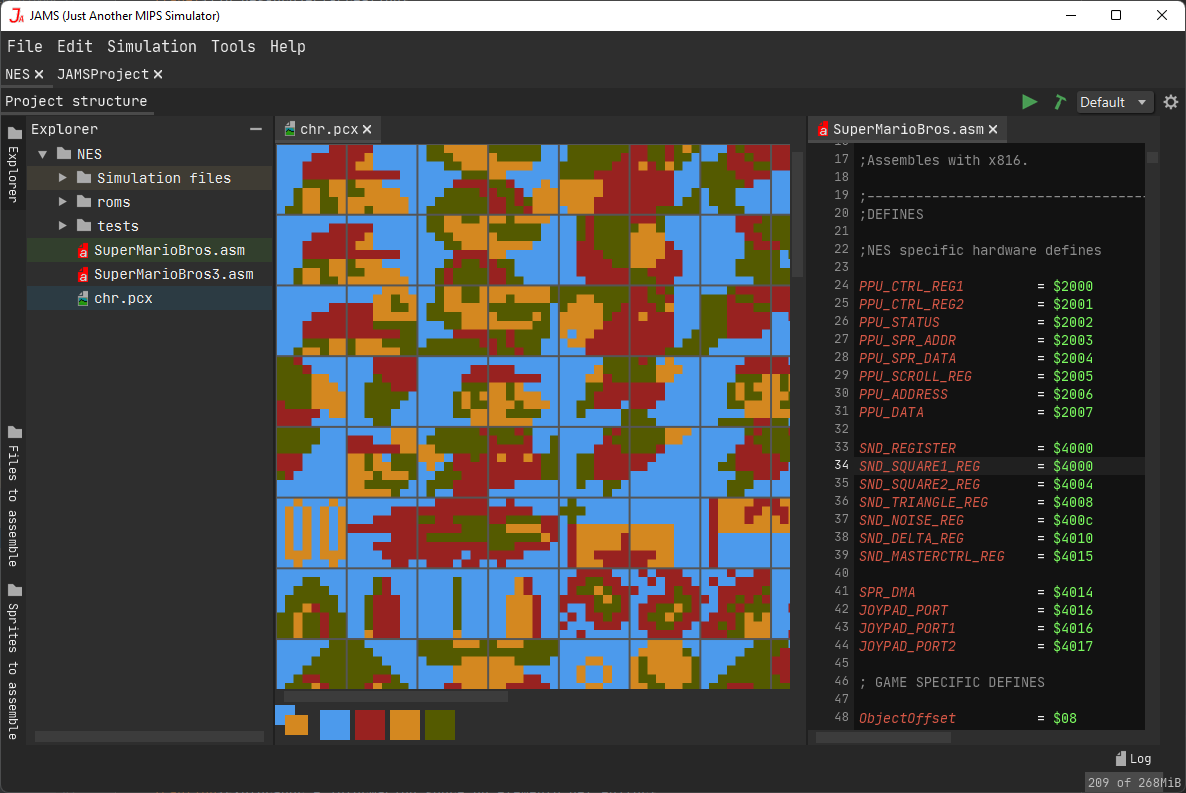
\includegraphics[width=0.8\textwidth]{images/nes/nes-editor}
    \caption{Editor de código y de gráficos junto con el explorador}
    \label{fig:nes-editor}
\end{figure}

El menú contextual del explorador presenta varias acciones que
pueden ejecutarse sobre las carpetas y los archivos
del proyecto.
Una de las opciones más particulares es la opción de añadir o eliminar
archivos de código o de gráficos del ensamblador.
Al ser \textit{JAMS} un entorno de desarrollo basado en \textbf{proyectos},
es necesario proporcionar una manera de incluir o excluir archivos del
videojuego resultante.
Con este sistema tan sencillo, el usuario podrá elegir qué archivos es preciso ensamblar.
Estos archivos para ensamblar estarán marcados en \textbf{verde} en el explorador,
y aparecerán en orden en los nodos \textbf{Archivos para ensamblar} y
\textbf{\textit{Sprites} para ensamblar}.
Cabe destacar que, como se verá más adelante, el orden de ensamblaje
importa, por lo que esta herramienta permite ordenar los ficheros de una manera sencilla.

Una vez el usuario abra un archivo, su editor aparecerá en la herramienta
principal de la sección: \textbf{el visualizador de archivos}.
\textit{NES4JAMS} añade dos editores nuevos a \textit{JAMS}:
el editor de código \textit{MOS 6502} y el editor de gráficos \textit{PCX}.

\subsection{Editor de código}\label{subsec:editor-de-codigo}

El editor de código usa el sistema de indexación desarrollado
en la capa base de \textit{JAMS}, por lo que este editor también
puede considerarse un \textbf{editor de texto inteligente}:
el editor convierte el texto puro en los componentes ensamblador
representados, pudiendo así aportar ayudas al usuario.
El editor también tiene conocimiento de las referencias y el alcance de
todas las etiquetas y macros, tanto en el propio archivo editado
como en el resto de archivos fuente del proyecto.
El editor también incorpora un \textbf{autocompletador}.
Esta herramienta ayuda al usuario cuando escribe código
aportando sugerencias de autocompletación, como se puede
observar en la figura \ref{fig:nes-autocompletion}.

\begin{figure}[h]
    \centering
    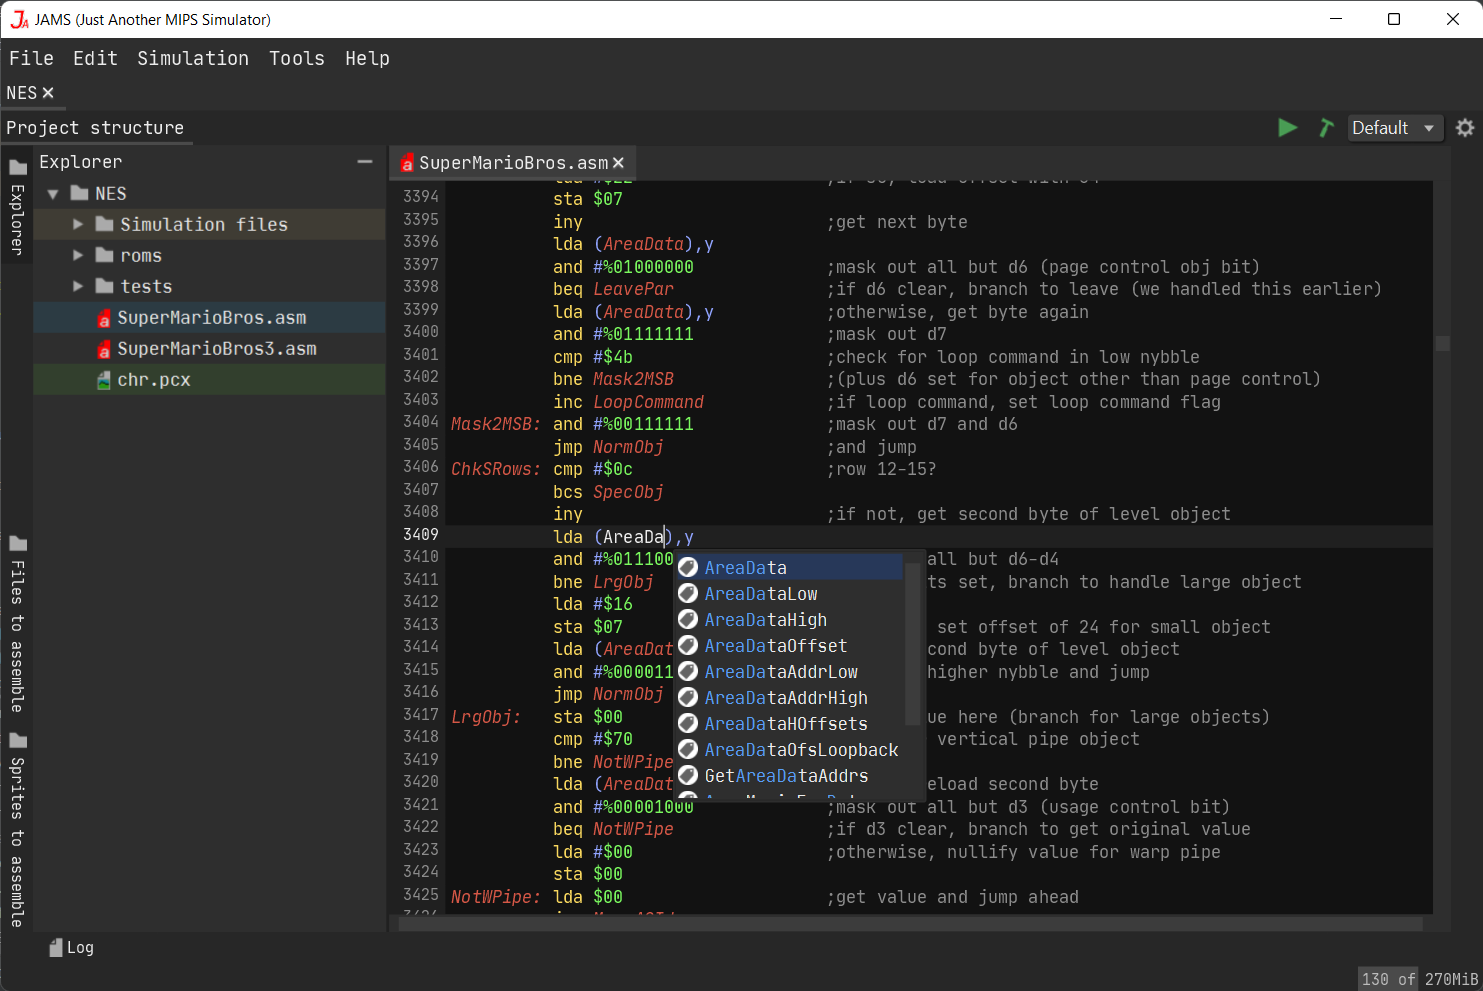
\includegraphics[width=0.8\textwidth]{images/nes/nes-autocompletion}
    \caption{Autocompletador ayudando al usuario}
    \label{fig:nes-autocompletion}
\end{figure}

\subsection{Editor de gráficos}\label{subsec:editor-de-graficos}

El editor de archivos \textit{PCX} permite modificar los
gráficos del videojuego de una manera rápida y sencilla.
Este editor está pensado exclusivamente para gráficos
de \textit{NES} (patrones a los que se les aplica una
paleta de cuatro colores), por lo que cada pixel solo puede tomar
cuatro valores diferentes.
El color final se buscará en la paleta seleccionada.
El usuario puede cambiar el color de cada elemento de la
paleta utilizando el botón central del ratón sobre
la entrada seleccionada.
Por motivos de accesibilidad, el usuario también puede
cambiar el color empleando el botón principal del
ratón mientras mantiene pulsada la tecla $Ctrl$.

Cabe destacar que, aunque este editor permite editar
archivos \textit{PCX} de cualquier tamaño, la consola
leerá el archivo como si tuviera un ancho de 128 píxeles.
Esto es debido a que las tablas donde se guardan los gráficos
en la consola tienen un tamaño de 16x16 patrones
de 8x8 píxeles cada uno.
Si se ensambla un archivo \textit{PCX} con otro ancho,
lo más probable es que los gráficos se conviertan en
\textbf{ruido}.
Los archivos \textit{PCX} creados por \textit{NES4JAMS}
siempre tienen el tamaño de una tabla de patrones,
es decir, de 128x128 píxeles.

\begin{figure}[h]
    \centering
    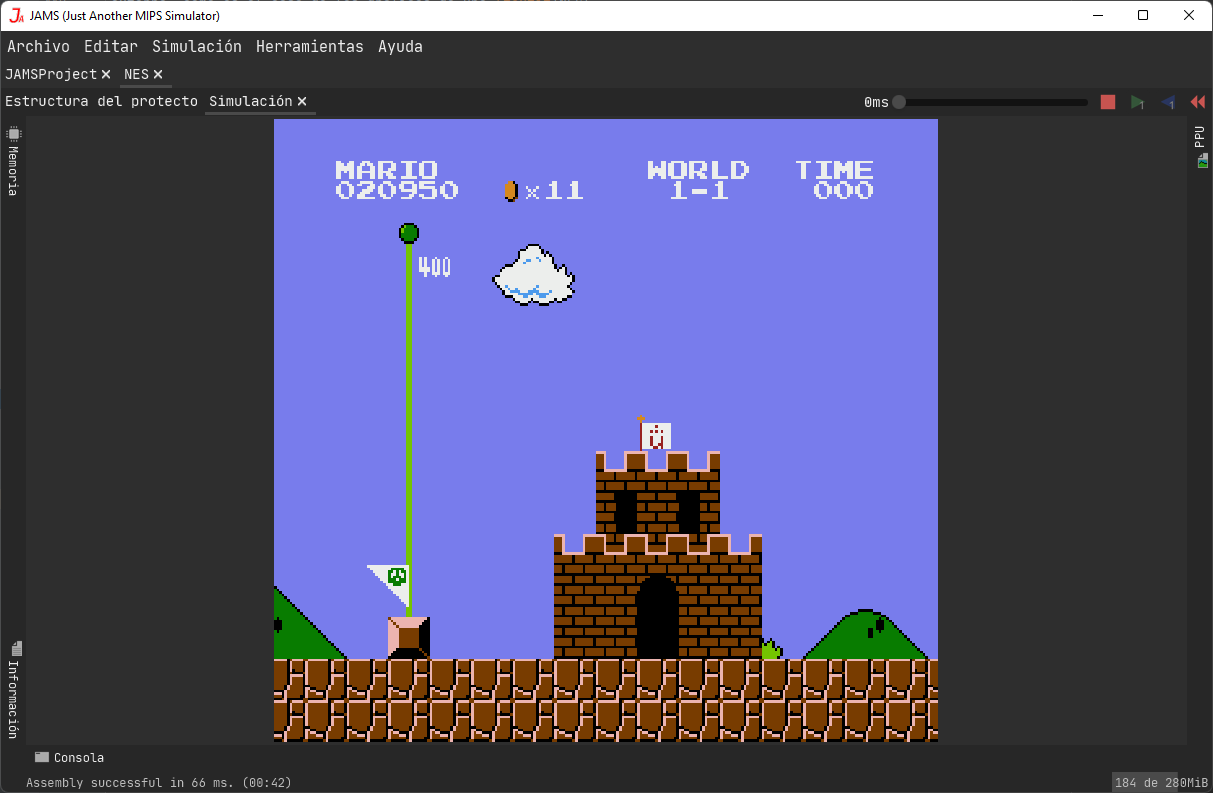
\includegraphics[width=0.8\textwidth]{images/nes/nes-graphics-change}
    \caption{\textit{Super Mario Bros.} con los gráficos modificados}
    \label{fig:nes-graphics-change}
\end{figure}

\subsection{Archivos iNES}\label{subsec:archivos-nes}

Como ya se comentó en los antecedentes,
el formato \textit{iNES} es el formato de archivo más utilizado
para almacenar videojuegos para la consola \textit{NES}.
Los archivos con este formato están divididos en tres secciones:
la cabecera, región del programa (\textit{PGR}) y la región de gráficos (\textit{CHR}).

\textit{NES4JAMS} es capaz de \textbf{cargar y generar} archivos
\textit{iNES} de manera nativa.
Al abrir un archivo \textit{iNES}, \textit{NES4JAMS} mostrará
el editor mostrado en la figura \ref{fig:nes-ines-editor}.

\begin{figure}[h]
    \centering
    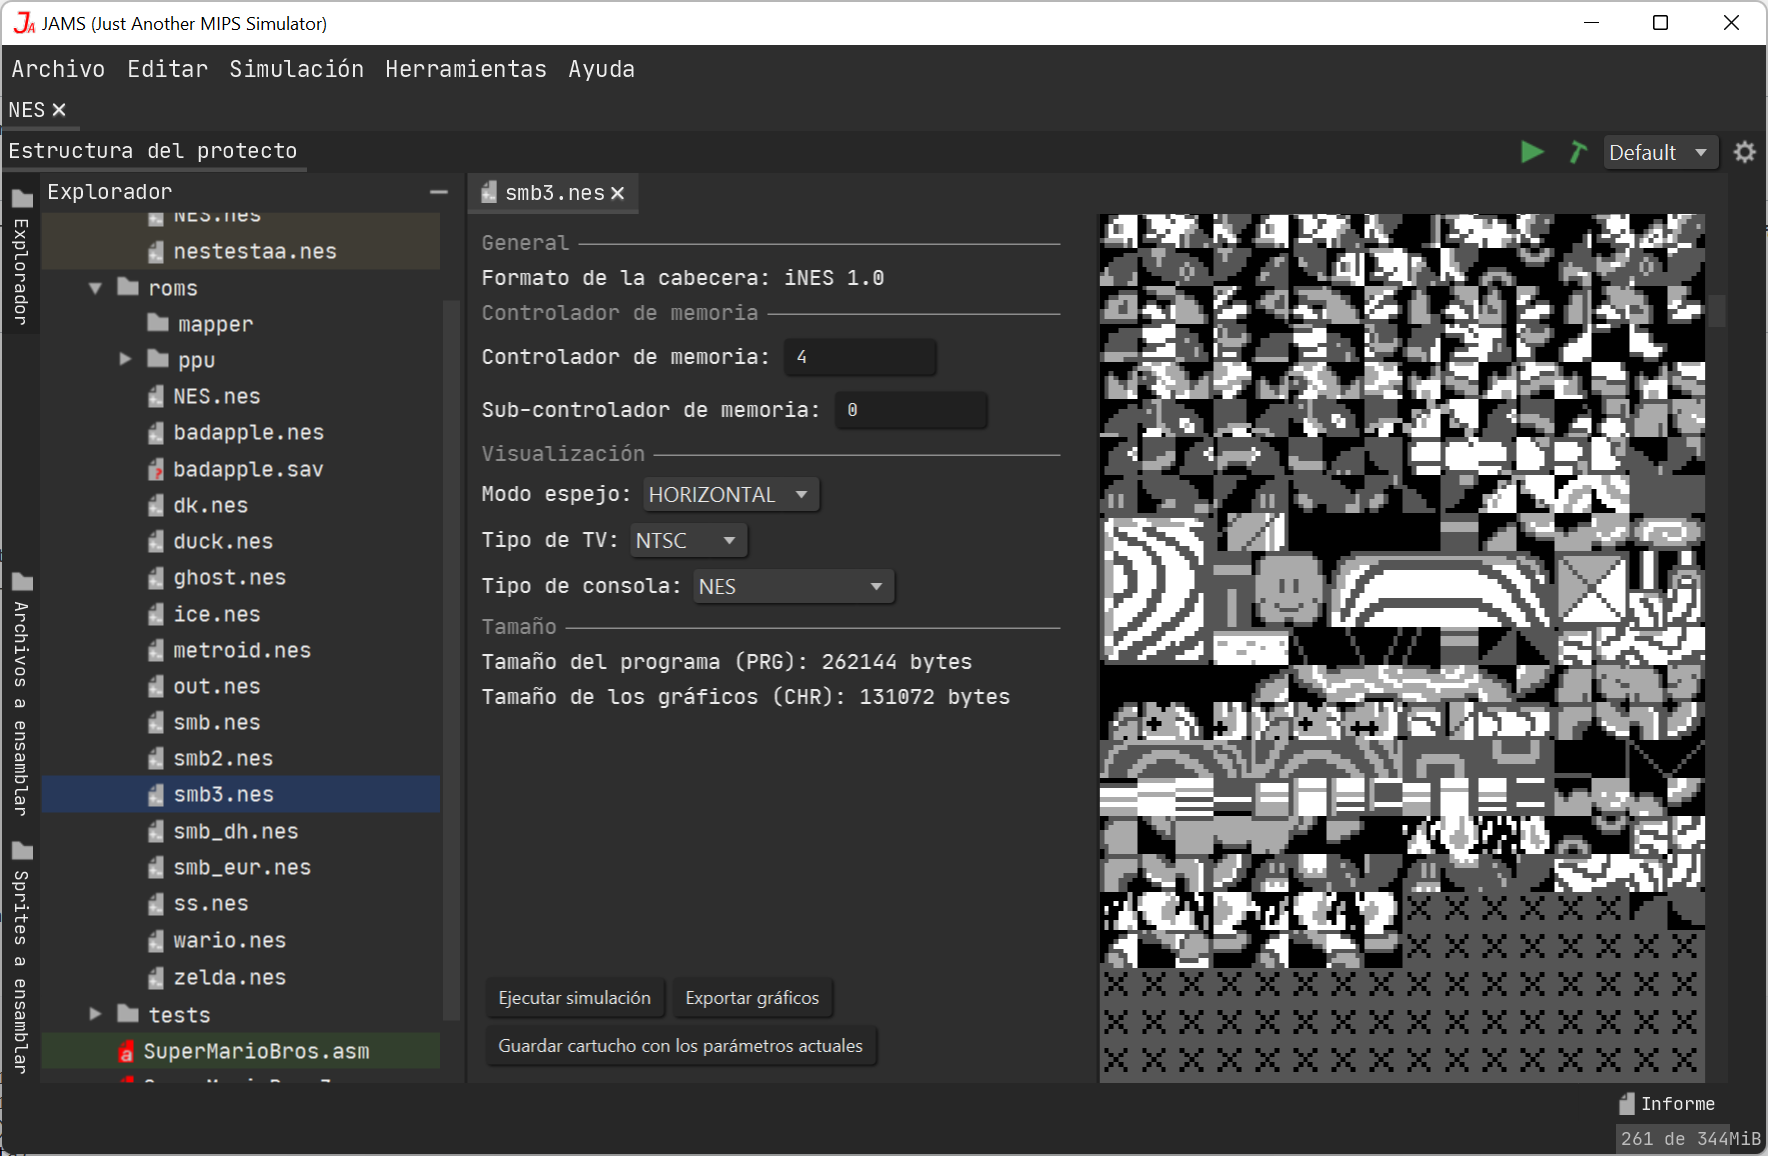
\includegraphics[width=0.8\textwidth]{images/nes/nes-ines-editor}
    \caption{Archivo \textit{iNES} en el editor}
    \label{fig:nes-ines-editor}
\end{figure}

En este editor el usuario podrá ejecutar una simulación
para el videojuego seleccionado, permitiéndole \textbf{modificar}
parámetros de cabecera.
El usuario también tiene la opción de \textbf{exportar las tablas
de patrones} del cartucho en un archivo \textit{PCX}.
Se puede observar una previsualización de estas tablas en la parte derecha del editor.
Por último, el editor ofrece la opción de \textbf{guardar una copia}
del videojuego con los parámetros modificados.

\subsection{Configuraciones}\label{subsec:configuraciones}

\begin{figure}[h]
    \centering
    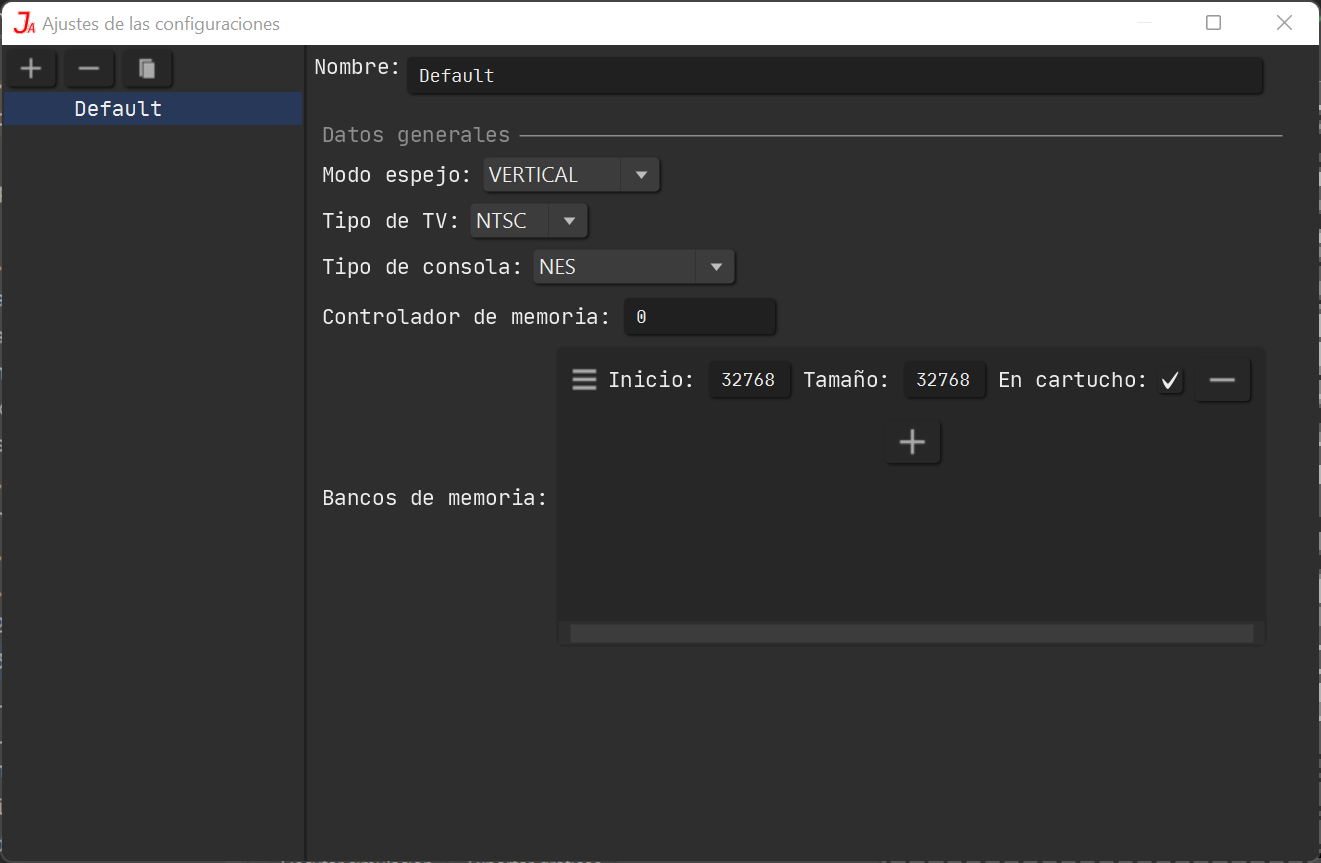
\includegraphics[width=0.8\textwidth]{images/nes/nes-configurations}
    \caption{Menú de configuraciones}
    \label{fig:nes-configurations}
\end{figure}

Igual que en el entorno de desarrollo para \textit{MIPS32},
el entorno de desarrollo \textit{NES} permite ensamblar
el programa con diferentes \textbf{configuraciones}.
Estas configuraciones definen los \textbf{parámetros de la cabecera}
del archivo \textit{iNES} resultante y los \textbf{bancos de memoria}
presentes en el cartucho.

Los bancos de memoria están definidos por una \textbf{dirección de inicio}
y un \textbf{tamaño} en bytes.
De manera muy similar a las directivas \textit{.text}
y \textit{.data} de \textit{MIPS32}, el desarrollador podrá
alternar entre bancos de memoria usando la directiva \textit{.bank}.

\textit{NES4JAMS} también incorpora una opción que impide copiar un
banco de memoria en el cartucho.
Esta funcionalidad es muy importante para algunos videojuegos
avanzados, ya que les permite utilizar un banco de memoria como
una representación de una \textbf{memoria RAM} adicional
dentro del cartucho.

La interfaz usada para modificar estas configuraciones puede observarse
en la figura \ref{fig:nes-configurations}.


\section{Ensamblador \textit{MOS 6502}}\label{sec:ensamblador}

El ensamblador para el procesador \textit{MOS 6502} se utiliza
para convertir los proyectos en archivos \textit{iNES}.
Este ensamblador soporta características avanzadas empleadas
comúnmente al programar, como las macros,
las etiquetas globales o las referencias relativas.
El código fuente de un proyecto se ensambla en \textbf{cuatro pasos}:
descubrimiento, expansión, asignación de direcciones y asignación de valores.
Estos son los mismos pasos que utiliza el ensamblador para \textit{MIPS32},
y es que el del \textit{MOS 6502} presenta \textbf{la misma arquitectura}
que el incluido por defecto en \textit{JAMS}.

\subsection{Descubrimiento}\label{subsec:descubrimiento}

En este paso el texto del proyecto se \textbf{descompone en sus primitivas},
permitiendo al ensamblador descubrir los diferentes componentes de cada línea.
Al final de este paso, las etiquetas globales y las etiquetas del archivo
(etiquetas no definidas dentro de una macro) \textbf{son registradas sin
ningún valor asignado}.
También se registran las macros de cada archivo.
El identificador de una macro es definido por su nombre concatenado
al número de parámetros que necesitan.
Este procedimiento se realiza para dar soporte a la sobrecarga de macros.
En el caso de la macro $print$, su identificador sería
$print-1$.

Cabe destacar que, a diferencia del ensamblador para \textit{MIPS32},
las etiquetas pueden hacer referencia a una dirección de memoria
o a una \textbf{equivalencia}.
Estas equivalencias relacionan una etiqueta con una expresión matemática
que a la vez puede hacer uso de otras etiquetas para calcular su valor.

\subsection{Expansión}\label{subsec:expansion}

En este paso, se invocan las llamadas a macro,
insertando el código de la macro en la posición de la llamada.
Este código efectúa el primer paso del ensamblaje mientras es añadido.
Al insertarse justo después de la llamada, el código de la macro
también será expandido.

\subsubsection{Alcance}\label{subsubsec:alcance}

Las etiquetas y macros que están dentro de una macro
\textbf{tienen un alcance diferente al del archivo}.
Si la macro es global, el alcance es considerado hijo del alcance global
y no podrá acceder a las etiquetas del archivo que lo invoca.
Si la macro es local, el alcance es considerado hijo del alcance del archivo.

Cuando un alcance es hijo de otro alcance,
\textbf{el hijo podrá acceder a las etiquetas y macros de su padre}.
El hijo también podrá definir nuevas etiquetas y macros con el mismo
identificador que una etiqueta o macro de su padre.
Aunque este comportamiento está permitido, \textbf{el hijo solo podrá acceder
al elemento que él define}.
Esta funcionalidad es llamada \textbf{ocultamiento o \textit{shadowing}}.

\subsection{Asignación de direcciones}\label{subsec:asignacion-de-direcciones}

Una vez el ensamblador haya expandido las macros,
se asignan las direcciones de todas las instrucciones,
etiquetas y directivas que lo requieran.
Estas direcciones se asignan de manera secuencial.
Existen directivas que pueden modificar el flujo de la asignación,
como es el caso de la directiva $.bank$ anteriormente mencionada.

\subsection{Asignación de valores}\label{subsec:asignacion-de-valores}

Como paso final, el ensamblador insertará en memoria los valores
que representan las directivas e instrucciones.
Es en este paso donde se resuelven los valores de las equivalencias.

\subsection{Empaquetamiento}\label{subsec:empaquetamiento}

Como paso adicional fuera del ensamblador, los datos resultantes
en los bancos de memoria son empaquetados en un archivo \textit{iNES}.
Este archivo junta la cabecera especificada en la configuración seleccionada
por el usuario, los bancos de memoria especificados como memoria
\textit{ROM} y los gráficos traducidos a tablas de patrones.
Este archivo está situado en los archivos del simulador, lo que
permite que el desarrollador pueda distribuir su videojuego
y utilizarlo en otros emuladores.

\subsection{Características avanzadas}\label{subsec:características-avanzadas}

El ensamblador permite el uso de técnicas avanzadas en
el desarrollo de aplicaciones en lenguaje ensamblador, como
las que se detallan a continuación.

\begin{itemize}
    \item \textbf{Referencias relativas}: una directiva o instrucción puede \textbf{referenciar a una etiqueta de manera
    relativa} con las referencias especiales $+$ y $-$.
    La referencia $+$ hace referencia a la etiqueta siguiente.
    La referencia $-$ hace referencia a la etiqueta anterior.
    Las referencias relativas \textbf{solo pueden hacer referencia
    a etiquetas del mismo alcance}.
    No pueden hacer referencia a etiquetas de un alcance mayor.
    \item \textbf{Macros anidadas}: una macro puede ser definida dentro de otra macro.
    Esto es conocido como una \textbf{macro anidada}.
    Una macro anidada solo podrá ser accedida en el alcance de la macro
    en la que está declarada.
    \item \textbf{Expresiones}: las expresiones son la característica más avanzada
    presente en el ensamblador, y permite deducir el valor
    de una instrucción o directiva mediante una \textbf{expresión matemática}
    que puede usar etiquetas como parámetros.
    Los usuarios pueden emplear una gran variedad de operaciones
    en las expresiones, como son la suma, la resta, la multiplicación,
    la división y las operaciones lógicas a nivel de bit.
    También existen operaciones \textbf{unarias}, como son
    la conversión de un número en byte o palabra,
    la negación a nivel de bit o la selección del
    primer o segundo byte de una palabra.
    Estas expresiones se utilizan de manera directa en las
    instrucciones y directivas, como se observa en
    la figura \ref{fig:nes-expressions}.
\end{itemize}

\begin{figure}[h]
    \centering
    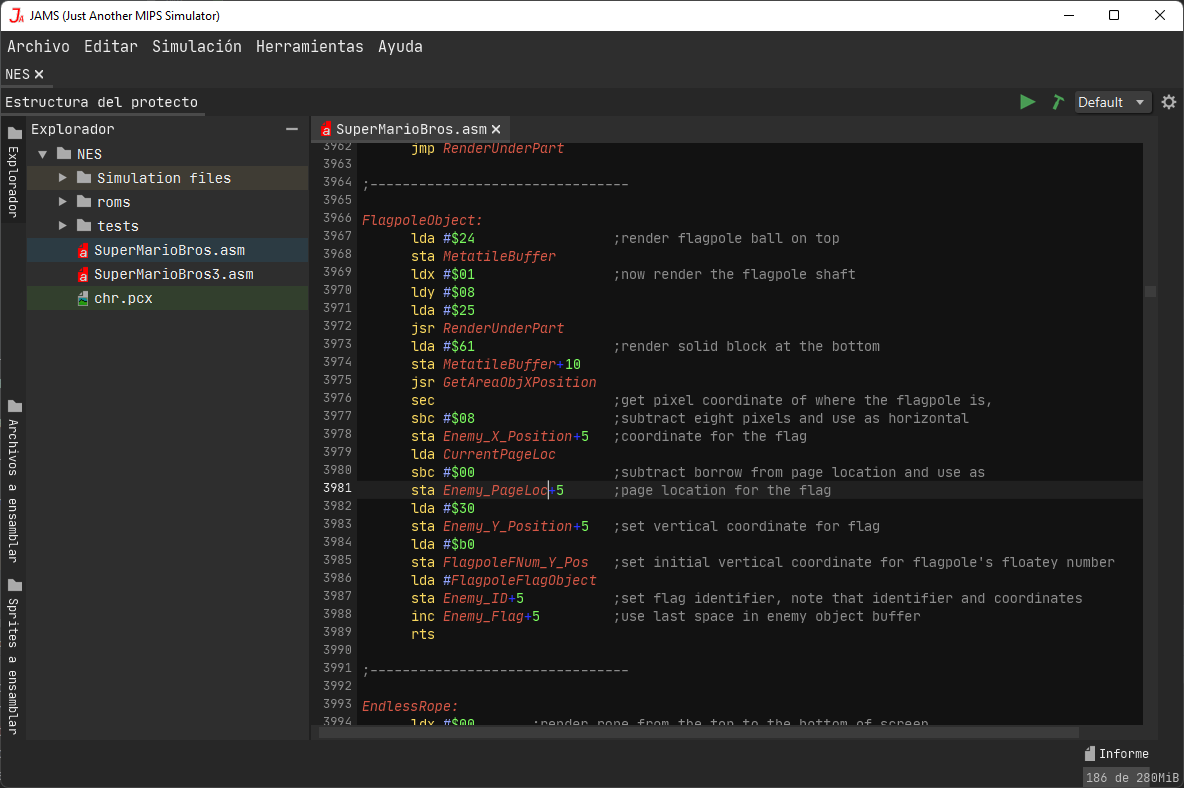
\includegraphics[width=0.8\textwidth]{images/nes/nes-expressions}
    \caption{Expresiones con sumas usadas en instrucciones}
    \label{fig:nes-expressions}
\end{figure}

\subsection{Detalles finales}\label{subsec:detalles-finales}

A diferencia del ensamblador para \textit{MIPS32},
este ensamblador no es muy personalizable.
Esto es debido a que \textit{NES4JAMS} pretende
ser un entorno de desarrollo de videojuegos para la \textit{NES}
que puedan ejecutarse en \textbf{consolas reales}.
\textit{NES4JAMS} da soporte para todas las
\textbf{instrucciones legales} presentes en la consola,
por lo que no es factible dar soporte para instrucciones
de terceros.


\section{Simulador}\label{sec:simulador}

Un simulador es una pieza de \textit{software} que imita el
comportamiento de un dispositivo.
\textit{NES4JAMS} introduce un simulador de la arquitectura
de la consola \textit{NES} que permite jugar y depurar
una gran variedad de videojuegos.

El simulador está principalmente compuesto por cinco partes:
la unidad central de procesamiento
(\textit{Central Processing Unit} o \textit{CPU}),
la unidad de procesamiento de imágenes
(\textit{Picture Processing Unit} o \textit{PPU}),
la unidad de procesamiento de audio
(\textit{Audio Processing Unit} o \textit{APU}),
el bus de datos y el controlador de memoria o \textit{mapper}.
El simulador simula el comportamiento de todos los componentes
en cada \textbf{ciclo de reloj}.

\subsection{Estructura del simulador}\label{subsec:estructura-del-simulador}

El nodo principal del simulador para la consola \emph{NES} no
es un visualizador de instrucciones, sino una herramienta que
simula la \textit{salida de vídeo} de la consola y que puede
observarse en la figura \ref{fig:nes-video}.

\begin{figure}[h]
    \centering
    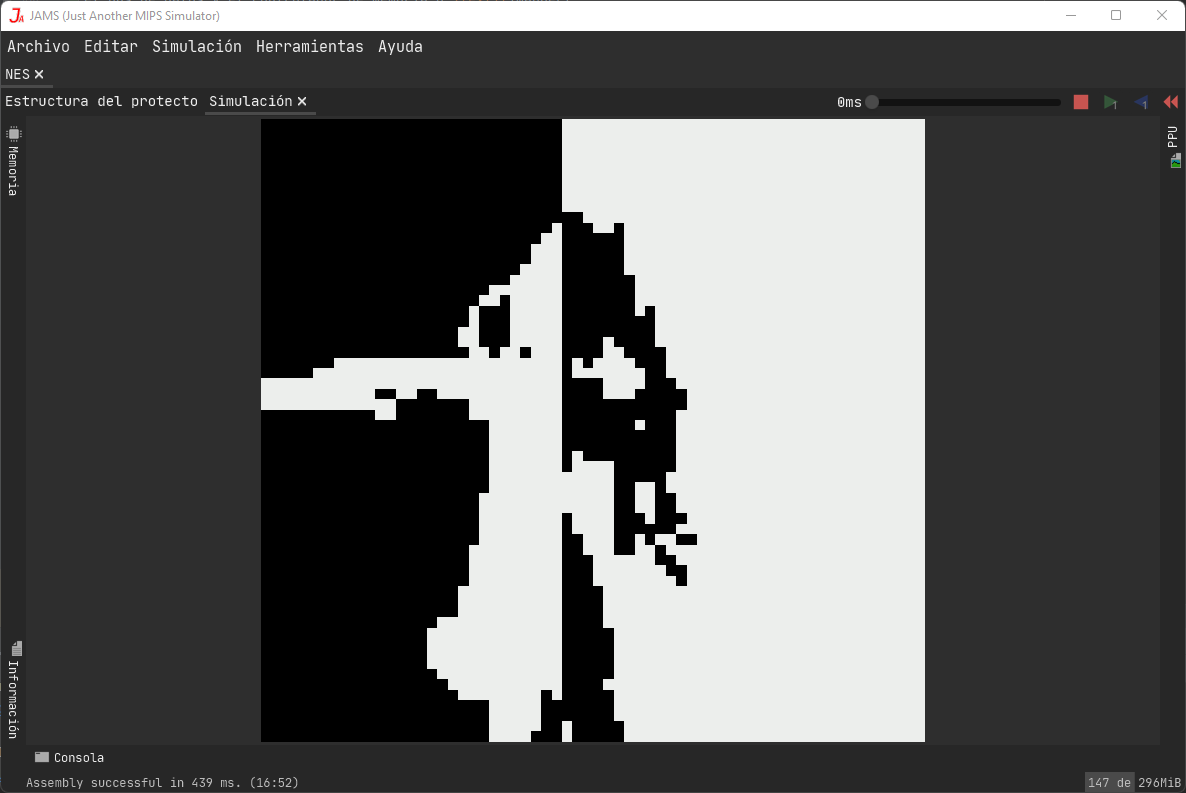
\includegraphics[width=0.8\textwidth]{images/nes/nes-video}
    \caption{Simulador reproduciendo una versión de \textit{Bad Apple!} para la \textit{NES}}
    \label{fig:nes-video}
\end{figure}

A diferencia de los cauces gráficos actuales, la \textit{NES}
compone la imagen de salida generando \textbf{un pixel} cada
ocho ciclos de reloj de la \textit{PPU}.
Este comportamiento, junto con otras características como
la generación de interrupciones de la unidad central
por parte de la propia \textit{PPU}, hace imposible usar
herramientas de renderizado avanzadas como las proporcionadas
por librerías como \textit{Vulkan} u \textit{OpenGL}.

La única manera de renderizar la salida de vídeo de la \textit{NES}
es generando la imagen en el \textbf{mismo hilo de ejecución}
utilizado por la \textit{CPU}.
De esta manera, la \textit{PPU} ejecuta una cantidad de ciclos
determinada por la región por cada ciclo de \textit{CPU}.

\textit{JavaFX} no está optimizada para modificar imágenes en movimiento.
La herramienta de vídeo emplea una versión \textbf{muy modificada}
de las imágenes proporcionadas por la librería,
permitiendo así modificar una imagen muchas veces por segundo
de manera constante.

Esta salida de vídeo se complementa con dos herramientas principales:
la herramienta \textit{memoria} y la herramienta \textit{PPU}.
Existen otras herramientas secundarias, como la \textit{consola}, que permite
visualizar el resultado de la simulación cuando se para, o
la \textit{información}, que permite visualizar el número de imágenes por segundo
mostradas en la salida de vídeo.

\subsection{Memoria}\label{subsec:memoria}

La memoria de la \textit{NES} puede separarse en \textbf{tres secciones}:
la memoria \textit{RAM}, la memoria del cartucho y la memoria \textit{VRAM}.
La memoria del cartucho está dividida en dos secciones:
la memoria del programa (\textit{PRG}), donde se guardan
las instrucciones del videojuego,
y la memoria de los gráficos (\textit{CHR}), donde se guardan
las tablas de patrones.
A su vez, la memoria \textit{VRAM} o \textit{RAM} de la \textit{PPU}
se divide también en dos secciones:
las tablas de nombres y las paletas de colores.

La consola presenta \textbf{dos buses de datos}:
el bus de datos de la \textit{CPU}
y el bus de datos de \textit{PPU}.
El bus de datos de la \textit{CPU} permite a
este acceder a la memoria \textit{RAM},
a los registros de la \textit{PPU},
a los registros de la \textit{APU}
y a la memoria \textit{PRG} del cartucho.
A su vez, el bus de datos de la \textit{PPU}
le permite a este acceder a las tablas de patrones
del cartucho, a las tablas de nombres y a las paletas
de colores.

La memoria de los cartuchos que visualizan la \textit{CPU}
y la \textit{PPU} suelen pasar por un controlador de memoria,
que está situado dentro de cada cartucho
de juego.
Existen más de 250 tipos de controladores, cada
uno con características específicas.
Al permitir la \textit{NES} poder realizar operaciones de
escritura en memoria del cartucho, los controladores
pueden utilizar \textbf{registros} internos que cambian
el comportamiento del cartucho.
Esta técnica se usa principalmente para \textbf{alternar
entre bancos de memoria}.

\begin{figure}[h]
    \centering
    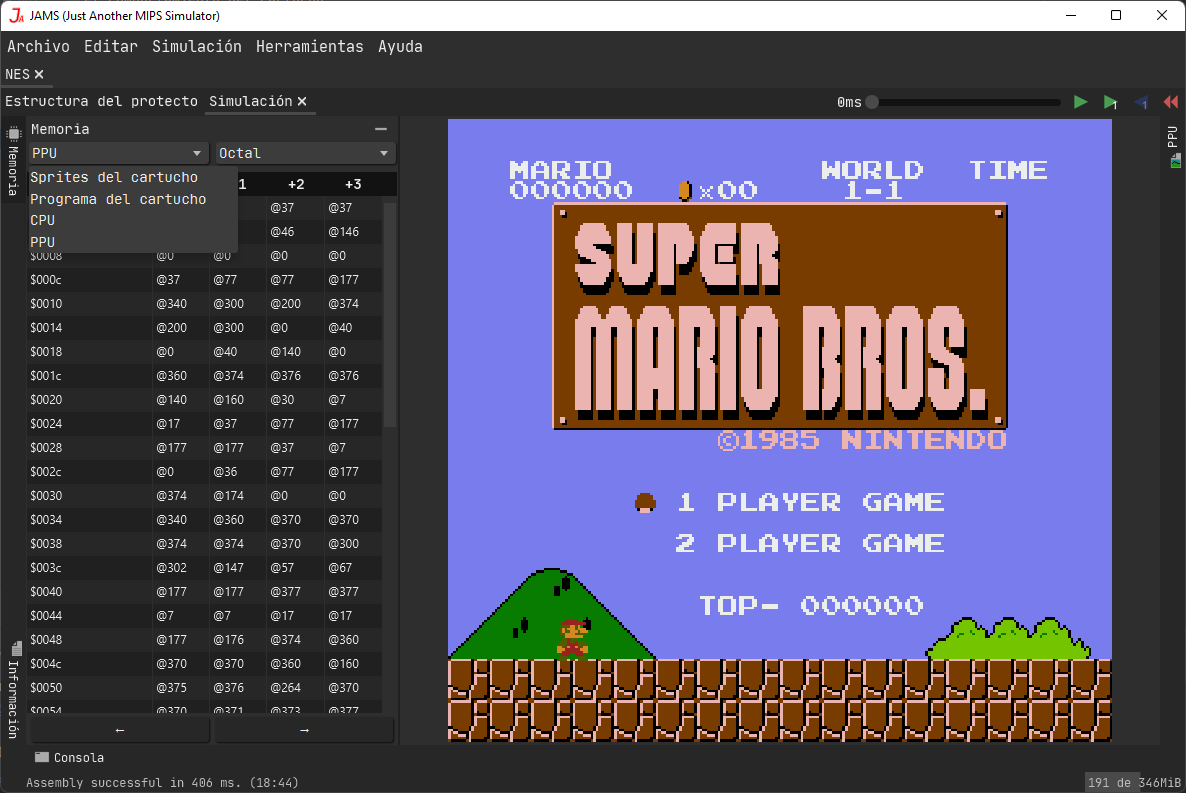
\includegraphics[width=0.8\textwidth]{images/nes/nes-memory}
    \caption{Memoria del simulador}
    \label{fig:nes-memory}
\end{figure}

La herramienta \textbf{memoria} mostrada en la
figura \ref{fig:nes-memory} permite
al usuario visualizar la memoria del simulador desde
el punto de vista de la \textit{CPU} de la \textit{PPU}.
Adicionalmente, también le permite visualizar los bancos
de memoria del cartucho de forma directa, sin controladores
de memoria de por medio.

El usuario también puede \textbf{escribir} valores en una
dirección de memoria.
Esta escritura se tratará como una escritura de la \textit{CPU}
o la \textit{PPU}, dependiendo del punto de vista seleccionado.
Por este motivo, existen escrituras realizadas desde uno de estos
dos puntos de vista que resultarán \textbf{sin efecto} alguno,
ya que se intentará modificar valores como los bancos de memoria
del cartucho, considerados como memoria de solo
lectura por ambos componentes.
Si el usuario desea modificar los bancos de memoria, puede
hacerlo desde la visualización directa.

\subsection{Unidad de procesamiento de imágenes}\label{subsec:unidad-de-procesamiento-de-imagenes}

La \textit{PPU}\cite{PPU} es la unidad de procesamiento encargada de generar
la salida de vídeo.
Debido a la escasa memoria presente en la \textit{VRAM}, la \textit{PPU}
está diseñada para ahorrar \textbf{la mayor cantidad de memoria posible}.
Esto lo consigue construyendo la escena mediante un complejo
sistema de paletas y tablas de patrones.

\subsubsection{Fondo de la escena}\label{subsubsec:fondo-de-la-escena}

Para generar el fondo de la escena, la \textit{PPU} utiliza
tres bancos de memoria diferentes: las tablas de patrones\cite{PATTERN_TABLES},
las tablas de nombres\cite{NAME_TABLES} y las paletas\cite{PALETTES}.

Las tablas de nombres tienen un tamaño de 32x32 bytes.
Las 30 primeras filas guardan el índice del patrón
utilizado en la posición asignada a dicha dirección.
Las dos últimas filas almacenan el identificador de las
paletas empleado en cada conjunto de 2x2 índices.
De esta manera se genera un escenario de 32x30 patrones.

La \textit{PPU} contiene en su memoria \textbf{dos tablas de nombre}
(comúnmente denominadas \textit{A} y \textit{B}),
aunque tenga reservado direcciones de memoria para cuatro de ellas.
Estas direcciones \textbf{apuntan} a la tabla
\textit{A} o a la tabla \textit{B} dependiendo
del \textbf{modo espejo}\cite{MIRRORING} especificado por el videojuego.
Cabe destacar que existen videojuegos con memoria \textit{RAM}
extra en sus cartuchos, permitiendo añadir las tablas \textit{C} y \textit{D}.

\begin{figure}[h]
    \centering
    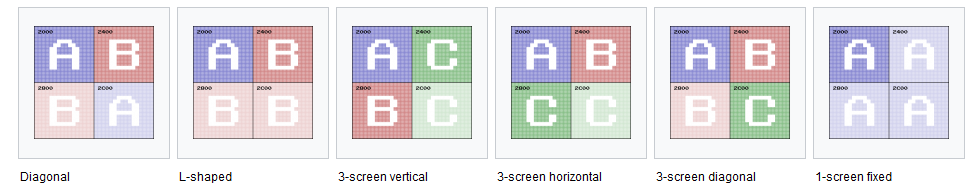
\includegraphics[width=\textwidth]{images/nes/nes-mirroring}
    \caption{Diferentes modos espejo representados en la web \textit{NESdev Wiki}}
    \label{fig:nes-mirroring}
\end{figure}

\begin{figure}[h]
    \centering
    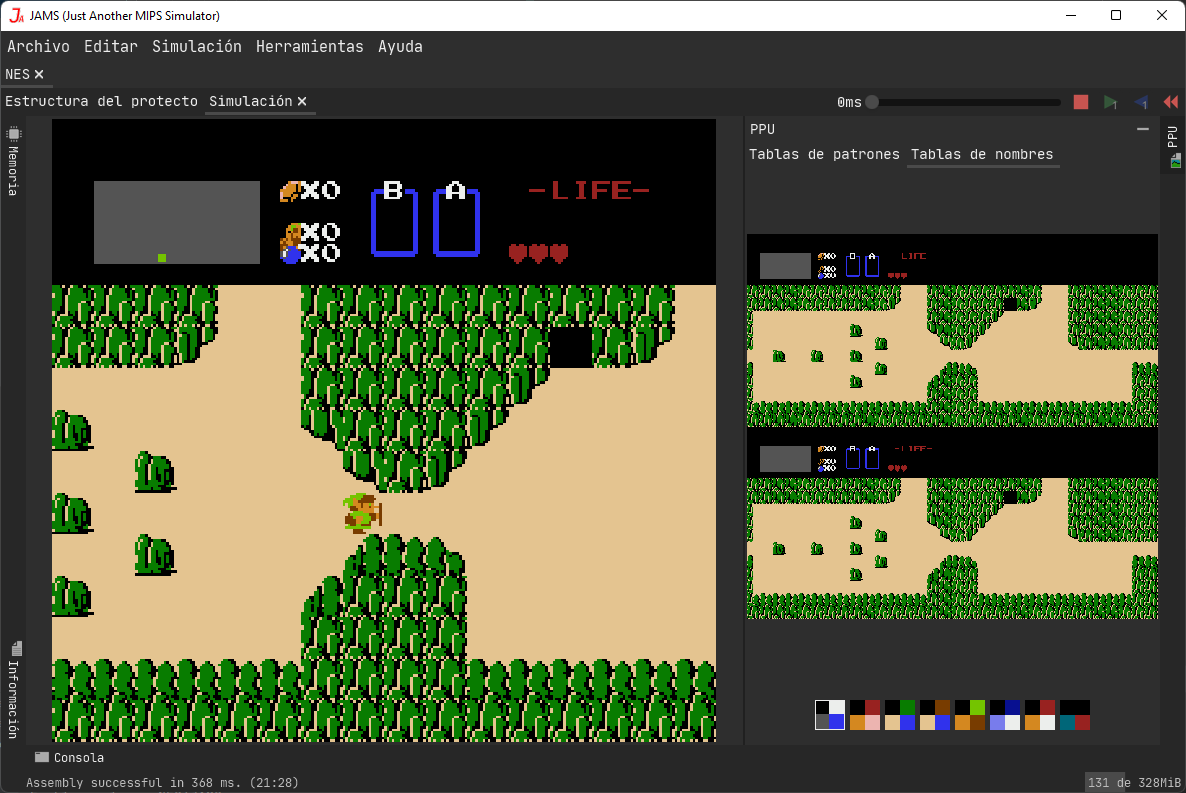
\includegraphics[width=0.8\textwidth]{images/nes/nes-nametables}
    \caption{Tablas de nombres en la herramienta \textit{PPU}}
    \label{fig:nes-nametables}
\end{figure}

Las tablas de patrones permiten guardar 16x16 patrones de
8x8 píxeles cada uno.
Cada pixel ocupa 2 bits de memoria, por lo que una tabla
de patrones ocupa 4 KiB.
La \textit{NES} presenta \textbf{dos tablas de patrones}, siendo
por defecto la primera utilizada para el fondo y la segunda
para los \textit{sprites}.

Por último, la \textit{NES} contiene \textbf{ocho paletas}
de cuatro colores cada una.
Las cuatro primeras paletas se usan para el fondo,
mientras que las cuatro últimas se emplean para los \textit{sprites}.
El primer color de las paletas tiene un comportamiento especial:
en las paletas de fondo, este color siempre es el mismo,
leyendo la \textit{PPU} siempre el color de la primera paleta.
Se considera este color como el color base de la escena.
En las paletas de los \textit{sprites}, el primer color
se considera siempre transparente.

Con esta configuración, la \textit{NES} genera una escena de juego
con un fondo de 512x480 píxeles, cuatro veces mayor que la salida
de vídeo de la consola.
La \textit{PPU} permite a los videojuegos desplazar la salida
de vídeo por la escena con una precisión de píxel.
Si el desplazamiento es tan grande que el área de renderizado
sale de la escena, se produce un desbordamiento en la \textit{PPU},
de forma que la tabla de nombres actúa como una memoria circular
y se dibuja en pantalla el fragmento de la escena que está en el lado contrario.
Gracias a estas propiedades se puede crear videojuegos con
un desplazamiento suave y fácil de implementar.

\subsubsection{\textit{Sprites}}\label{subsubsec:sprites}

La \textit{PPU} contiene una memoria exclusiva para guardar
los atributos de los \textit{sprites}.
Esta memoria recibe el nombre de \textit{OAM} u \textit{Object Attribute Memory}\cite{OAM},
y es capaz de almacenar hasta 64 \textit{sprites}.
Cada \textit{sprite} ocupa 4 bytes de memoria, donde se
definen atributos como el índice del patrón o la posición en la escena.

Cabe destacar la posición de los \textit{sprites} es
absoluta con respeto a la salida de vídeo, por lo que no
es afectada por el desplazamiento del fondo.
Es el propio videojuego el que debe encargarse
de actualizar la posición de todos los \textit{sprites}
cuando la escena se desplaza.

\subsubsection{Herramienta \textit{PPU}}

\begin{figure}[h]
    \centering
    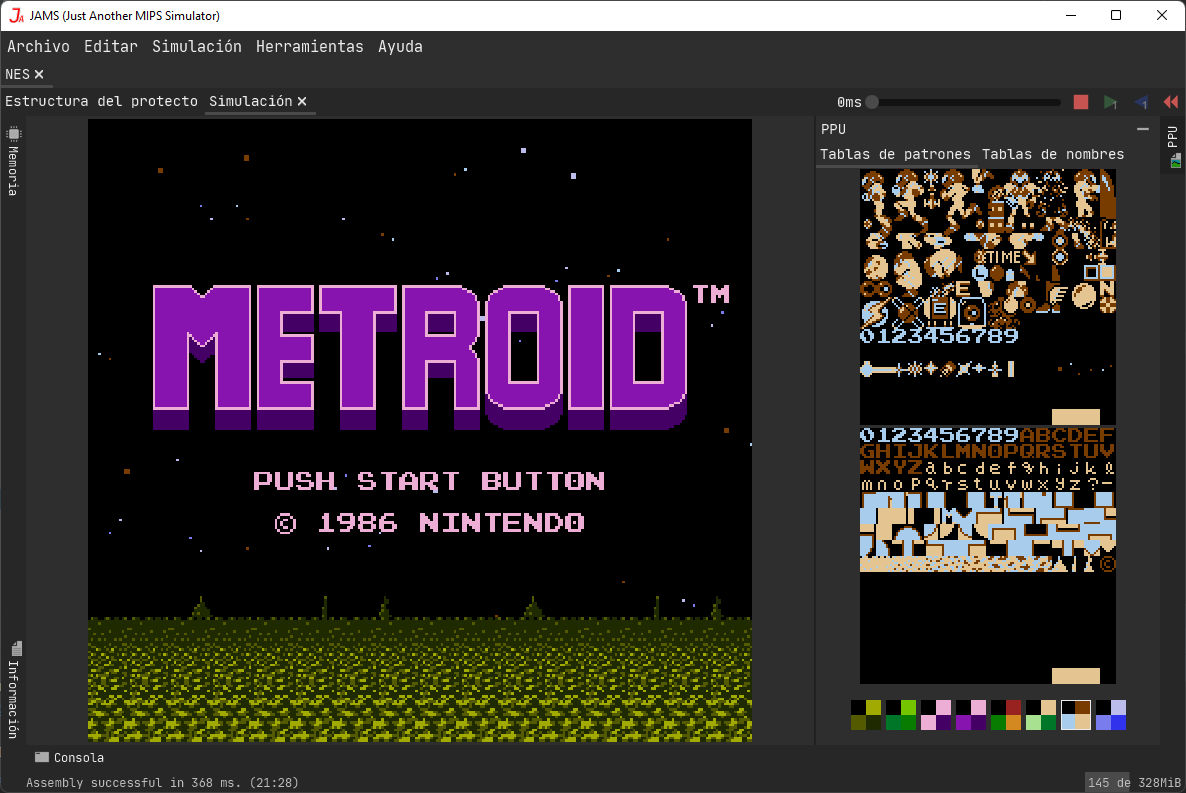
\includegraphics[width=0.8\textwidth]{images/nes/nes-patterntables}
    \caption{Paletas y tablas de patrones en la herramienta \textit{PPU}}
    \label{fig:nes-patterntables}
\end{figure}

La herramienta \textbf{PPU} del simulador permite
visualizar las tablas de patrones, las tablas de nombres
y las paletas que residen actualmente en memoria.
Estos datos se actualizan \textbf{en cada fotograma},
lo que permite detectar los cambios en la \textit{PPU}
de una manera muy visual.
Las figuras \ref{fig:nes-nametables} y \ref{fig:nes-patterntables}
muestran las diferentes opciones de esta herramienta.

Cabe destacar que esta herramienta no es puramente visual:
el usuario puede seleccionar una paleta de la lista.
Esto hará que las tablas de patrones \textbf{usen la paleta seleccionada}.
Muchos videojuegos modifican algunas paletas cada poco tiempo
para crear pequeñas animaciones.
Este es el caso de las monedas en \textit{Super Mario Bros.}, que
cambian de color cíclicamente.
Si la paleta seleccionada está siendo animada, las tablas de patrones
cambiarán de color de forma alternativa.

\subsection{Audio}\label{subsec:audio}

La consola \textit{NES} presenta
una \textbf{unidad de procesamiento de audio} o \textit{APU}\cite{APU}.
Esta unidad tiene \textbf{cuatro canales}: dos canales de pulso,
un canal triangular y un canal de ruido.

En la consola original, los cuatro canales generaban una muestra
por cada ciclo de reloj de la \textit{CPU}, lo que equivaldría
a \textbf{1,77 millones de muestras por minuto}.
Esta cantidad de muestras es innecesaria en un equipo de sonido
moderno, y su reproducción resulta inviable en las librerías
modernas.
Por ello \textit{NES4JAMS} rebaja la cantidad de datos comprimiendo
todas las muestras de un periodo de tiempo en una media ponderada.

\subsection{Unidad de procesamiento central}\label{subsec:unidad-de-procesamiento-central}

Como elemento final del simulador se encuentra el componente
principal de la consola: la \textbf{unidad de procesamiento central}
o \textit{CPU}.
La \textit{NES} usa un procesador \textit{MOS 6502}\cite{MOS6502}: una unidad
de procesamiento central de 8 bits muy utilizada a principio
de los años 80.

Aunque el número de instrucciones documentadas por \textit{MOS Technologies}
sea de 151, existen \textbf{instrucciones no oficiales}, producto del diseño
del procesador, lo que aumenta el número de instrucciones a 256.
\textit{NES4JAMS} actualmente \textbf{no soporta} este tipo de instrucciones,
lo que puede impedir simular ciertos juegos las utilizan.

